%=========================================================================
%DADOS DA INSTITUIÇÃO
\logoInst{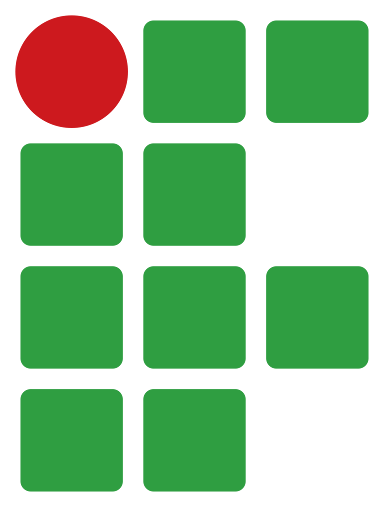
\includegraphics[width=0.4\textwidth]{./04-figuras/logoifba_capa}}

%======================================================================================================
%DADOS DO TRABALHO
%************************************************************************************
\titulo{Percepções e Adoção de TypeScript e JavaScript no Desenvolvimento Front-End: Um Estudo entre Iniciantes e Profissionais Experientes}
\titleenglish{Perceptions and Adoption of TypeScript and JavaScript in Front-End Development: A Study Among Beginners and Experienced Professionals}
%\subtitulo{Subtítulo do trabalho}
\autor{Gustavo da Silva Ferreira}
\tipotrabalho{Monografia} %troque por Tese (Doutorado) para tese de doutorado ou monografia se for o caso
\preambulo{Trabalho de Conclusão de Curso submetido ao Curso de Bacharelado em Sistemas de Informação, do campus de Feira de Santana do Instituto Federal da Bahia (IFBA), como um dos requisitos para a obtenção do título de Bacharel em Sistemas de Informação}
%===============================================================
%ORIENTAÇÃO DO TRABALHO
%*****************************************************************
\orientador{Prof Dr.Clerber Jorge Lira}  %Para orientadora:\orientador[Orientadora:]{Nome da orientadora}
%\coorientador{Prof. Dr. Sicrano Beltrano} %para coorientadora: \coorientador[Coorientadora:]{Nome da coorientadora}. Caso  tenha coorientador, descomente esta linha
%\instCoorientador{Universidade do Estadoda Bahia (UNEB)} %Necessário, pois o Coorientador pode ser de outra instituição (caso não seja, comente esta linha)
%\areaconcentracao{Modelagem Matemática e Computacional} %Não necessário no modelo 	UESC
%\linhapesquisa{Sistemas Inteligentes} %Não necessário no modelo UESC (caso necessário na sua intituição, descomente)
%========================================================================================================

%======================================================================================================
%DADOS DA INSTITUIÇÃO
%****************************************************************************************************
\instituicao{INSTITUTO FEDERAL DA BAHIA} %instituição
\campus{CAMPUS FEIRA DE SANTANA} % Se não tiver, deixe em branco
\curso{BACHARELADO EM SISTEMAS DE INFORMAÇÃO} %caso não queira colocar deixe em branco dentro das chaves
\programa{} %PARA PROGRAMAS DE PÓS GRADUAÇÃO-Especialização, mestrado ou doutorado. Por exemplo: Programa de Pós Graduação em Modelagem Computacional Em Ciência e Tecnologia
\local{FEIRA DE SANTANA-BA} %coloque o nome da cidade da sua instituição
\data{2025} %ano de defesa
%========================================================================================================

%======================================================================================================
%DADOS DA DEFESA
%****************************************************************************************************
%caso você não tenha coorienador comente a linha 38 do arquivo folhaAprovacao na pasta 01-Elementos-pre-textuais
\datadefesa{04/10/2024} %Coloque  data de defesa

\bancamembrointerno{Prof. Dr. Membro Interno} %Coloque o nome do membro interno que fará parte da banca
\bancainstmembrointerno{IFBA} %Coloque o nome ou sigla da instituição do membro interno que fará parte da banca

\bancamembroexterno{Prof. Me. Membro Externo} %Coloque o nome do membro externo que fará parte da banca
\bancainstmembroexterno{UESB} %Coloque o nome ou sigla da instituição do membro externo que fará parte da banca

